\documentclass[12pt,UTF8]{ctexbook}
\usepackage{ctex}
\usepackage{array}
\usepackage{graphicx}
\usepackage{wrapfig}
\usepackage[table,dvipsnames]{xcolor}
\usepackage{tabularx}
\usepackage{amsmath}
\usepackage{amssymb}
\usepackage{xfrac}
\usepackage{eucal}
\usepackage{titlesec}
\usepackage{amsthm}
\usepackage{tikz-cd}
\usepackage{enumitem}
\usepackage{verbatim}
\usepackage{caption}
\usepackage{fontspec,xunicode,xltxtra}
\usepackage{xeCJK} 
\usepackage[makeroom]{cancel}

% 修改脚注的编号为加圈样式,并且各页单独编号
\usepackage{pifont}
\usepackage[perpage,symbol*]{footmisc}
\DefineFNsymbols{circled}{{\ding{192}}{\ding{193}}{\ding{194}}
{\ding{195}}{\ding{196}}{\ding{197}}{\ding{198}}{\ding{199}}{\ding{200}}{\ding{201}}}
\setfnsymbol{circled}

\definecolor{gl}{RGB}{246, 252, 240}
\definecolor{gd}{RGB}{236, 244, 230}
\definecolor{bg}{RGB}{242, 244, 228}


\setCJKmainfont[BoldFont=STZhongsong]{STSong}
\setCJKmonofont{simkai.ttf} % for \texttt
\setCJKsansfont{simfang.ttf} % for \textsf
\setlength\parskip{8pt}
\setlength{\fboxsep}{12pt}
\renewcommand\thesection{\arabic{chapter}.\arabic{section}}
\newtheorem{df}{定义}[section] 
\newtheorem{pp}{命题}[section]
\newtheorem{tm}{定理}[section]
\newtheorem{ex}{例子}[section]
\newtheorem{et}{例题}[section]
\newtheorem{sk}{思考}[section]
\newtheorem{po}{公理}
\newtheorem*{so}{解答}
\newenvironment{proof2}{\paragraph{\textbf{证明:}}}{\hfill$\square$}
\newtheorem{xt}{习题}[section]
\newtheorem{cor}{推论}[pp]
% 列举环境的行间距
\setenumerate[1]{itemsep=0pt,partopsep=0pt,parsep=0pt,topsep=0pt}
\setitemize[1]{itemsep=0pt,partopsep=0pt,parsep=0pt,topsep=0pt}
\setdescription{itemsep=0pt,partopsep=0pt,parsep=0pt,topsep=0pt}
% 章节字体大小
\titleformat{\section}{\zihao{-2}\bfseries}{ \thesection }{16pt}{}
% 封面
\title{\zihao{0} \bfseries 第一册}
\author{\zihao{2} \texttt{大青花鱼}}
% \date{\bfseries\today}
\date{}
% 正文
\begin{document}
\maketitle
\tableofcontents
\newpage

\chapter{从自然数到有理数}

\section{分数、整数、有理数}
我们已经学过自然数:$0,1,2,3,\cdots$。自然数是$0$和$1$相加得到的数。
从$0$开始,不断加$1$,就能得到任何自然数。

比如:$4 = 0 + 1 + 1 + 1 + 1$。

自然数之间做加法和乘法,得到的还是自然数。

加法和乘法都满足结合律和交换律,乘法满足对加法的分配律。

自然数是自然产生的。当人们发现两头牛和两天有共同之处时,自然数的概念就诞生了。

为了回答类似“三个人分七只鸡”的问题,人们发明了除法。
除法是乘法的逆运算。

比如:$3 \times 7 = 21$,于是$3 = 21 \div 7$,$7 = 21 \div 3$。

除法产生了分数。自然数可以看作分母是$1$的分数。
分数之间可以做加法、乘法和除法,得到的还是分数。

为了回答类似“五个鸡蛋吃了两个还剩几个”的问题,人们发明了减法。减法是加法的逆运算。

比如,$3+2=5$,于是$3 = 5 - 2$,$2 = 5 - 3$。

既然可以写出$5-2$,那么可不可以写$0-2$呢?$0-2$有什么含义呢?

借用“五个鸡蛋吃了两个还剩几个”的思路,$0-2$可以表示“本没有鸡蛋,借来两个鸡蛋吃了两个还剩几个”。
这里剩下的,是“欠两个鸡蛋”,是一种负债状态。因此,这样的数称为\textbf{负数}。

我们一般把$0-2$中的$0$去掉,只记为$-2$。$-2$满足$-2+2=0$。对某个数,比如$73$来说,$73+(-2)=73+(0-2)=73-2$。
也就是说,一个数加上$-2$,就和减去$2$一样。以此类推,可以得到:
$$ -1, -2, -3, \cdots $$
它们由$1,2,3,\cdots$前加上减号得到,表示$0$减去$1,2,3,\cdots$的结果,读作“负一”、“负二”、“负三”等等。
我们把负数带的减号称为\textbf{负号}(读作“负”),和一般减法区别开来。

一般来说,在任何分数前加上负号,也可以得到一个负数,表示$0$减去它的结果。

有没有$-0$呢?$-0$就是$0-0$,也就是$0$自己,所以就没有必要加负号了。

自然数和它们的负数合称\textbf{整数}。我们把$-1, -2, -3, \cdots$这些负数称为\textbf{负整数},
把原来$1,2,3,\cdots$这些数称为\textbf{正整数},和负整数相对。由于$-0$就是$0$,约定$0$既不是正数,也不是负数。
于是整数分为正整数、负整数和$0$。

分数和它们的负数合称\textbf{有理数},我们把带负号的分数称为\textbf{负有理数}或\textbf{负分数},
把原来的分数(除了$0$)称为\textbf{正有理数}或\textbf{正分数}。
正有理数包括正整数,负有理数也包括负整数,有理数包括整数。

自然数或分数前面加负号得到的负数,叫做它的\textbf{相反数}。
反过来,一个负整数或负数去掉负号得到的数,也叫做这个它的相反数。
约定$0$的相反数就是$0$。于是,每个有理数都有唯一的相反数。

除了$0$以外,相反数总是成对的。一个有理数的相反数的相反数,就是它自己。

\begin{sk}\label{sk:0-0-0}
    一个有理数前面加上负号,一定会得到一个负数吗?
\end{sk}

加上一个负数,就和减去它的相反数一样。所以,现实问题中遇到和加法对应的具体概念,都可以用减法和负数表示相反或相对的概念。
比如,如果把“往东走三步”视作“$+3$”,那么“往西走两步”就可以视作“$-2$”。“原地往东走三步,再往西走两步”,就可以视作
“$0+3-2$”。计算得到$1$,就表示最终和原来比,往东走了一步。

\section{有理数的大小}
加法不仅可以表达累加的概念,还可以用于比较大小。比如,$5$比$3$大,$3$比$5$小。

我们用大于号“$>$”和小于号“$<$”记录大小关系。$5$比$3$大就写作$5>3$,读作“$5$大于$3$”;
$3$比$5$小就写作$3<5$,读作“$3$小于$5$”。

大小关系有哪些基本性质呢?

首先,大小关系用来形容不相等的数。所有不相等的数都能比大小。
两个数如果不相等,那么总有一个比较大,另一个比较小。

大小关系是\textbf{互反}的。说一个数比另一个数大,就是说另一个数比它小。反之亦然。

大小关系还是可以\textbf{传递}的,甲数比乙数大(小),乙数比丙数大(小),那么甲数就比丙数大(小)。

$5$比$3$大,可以理解为$5$是$3$再加自然数$2$得到的,
而$3$却没法通过$5$加上一个自然数得到。一般来说,如果一个数加上某个自然数或分数等于另一个数,
那么它比另一个数小,另一个数比它大。

我们希望大小关系对所有的有理数都成立,这样,我们就可以比较任何有理数的大小。首先,任何正有理数都大于$0$。
负有理数的相反数是分数,而任何负有理数加上它的相反数都得到$0$。
所以,按照大小关系的定义,我们规定$0$大于任何负有理数。于是任何正有理数大于$0$,从而大于任何负有理数。

我们约定大于$0$的数叫做\textbf{正数},小于$0$的数叫做\textbf{负数}。
正整数、正有理数都是正数,负整数、负有理数都是负数。
这样的约定和前面负数的定义是一致的。
之前的结论可以这么说:\textbf{任何正数大于任何负数}。

负有理数之间如何比较大小呢?举例来说,$0 = -3 + 3 = -3 + 1 + 2$,所以$-3 + 1 = 0 - 2 = -2$。
$-2$由$-3$加上自然数$1$得到,所以$-3$小于$-2$。进一步分析,我们发现,自然数$1$来源于“$3$可以写成$2+1$”。
所以我们可以总结出两个负有理数比较大小的方法:看它们的相反数。相反数中较大的,可以写成较小数加上一个分数,
于是,相反数较大的负有理数加上这个分数,就等于相反数较小的负有理数。因此,\textbf{相反数较大的负有理数比较小,
相反数较小的负有理数比较大}。

正数和负数可以比较大小。所以,现实问题中涉及到相反或相对的概念比较大小时,可以用有理数表示。

比如,今天延安的气温是$3.4$摄氏度,长春的气温是$-8.2$摄氏度,哈尔滨的气温是$-15.1$摄氏度,那么延安气温最高,
长春气温比延安低,而哈尔滨气温又比长春低。

\begin{sk}\label{sk:0-1-0}
    \mbox{}\\
    \indent 1. 用自己的话总结:我们是怎样定义负数的大小关系的?\\
    \indent 2. 怎么评价这样定义的大小关系?
\end{sk}

\section{乘方}
乘法可以更方便地表示若干个相同的数相加。比如,我们用$3 \times 4$表示$3+3+3+3$。
那么,能不能方便地表示若干个相同的数相乘呢?

我们把$3\times 3$称为$3$乘$2$\textbf{次方},把$7\times 7\times 7\times 7\times 7$称为$7$乘$5$次方。

同一个数连乘几次,叫做它乘几次方。连乘的结果,叫做它的几\textbf{次方}或几\textbf{次幂}。这种运算叫做\textbf{乘方}或\textbf{乘幂}。

我们把$7$的$5$次方记作$7^5$,把$7$称为\textbf{底数},把$5$称为\textbf{指数}。
这样记法,比$7\times 7\times 7\times 7\times 7$更方便。

一个数的$1$次方就是它自己。一个数的$2$次方也叫做它的\textbf{平方}。一个数的$3$次方也叫做它的\textbf{立方}。

约定任何数的$0$次方是$1$。

$7\times 7\times 7\times 7\times 7 = (7\times 7\times 7)\times (7\times 7)$。
用乘方表示这个关系,就是:$7^5 = 7^3 \times 7^2$。注意到$5 = 3 + 2$。
用日常的话来说,$5$个$7$相乘,等于$3$个$7$相乘,再和$2$个$7$相乘。

同底数乘方的积,是指数之和的乘方。乘方的乘法,可以转化为指数的加法。
因此,乘方的除法,也可以转化为指数的减法。

比如,$7^3 \times 7^2 = 7^{3+2} = 7^5$,所以,
$$7^{5-2} = 7^3 = 7^5 \div 7^2.$$
同底数乘方的商,是指数之差的乘方。

既然乘方的乘除可以转化为指数的加减,那么是否有负指数?能否定义一个数的负数次方?

如果定义$7^{-3}$为:$7^{-3} \times 7^3 = 7^{0} = 1$,那么
$7^{(-3)}$就等于$\frac{1}{7^3}$。一个数的负几次方,就是$1$除以它的几次方。

显然,$0$没有负数次方。

再来看乘方的乘方。考虑$\left(2^3\right)^4$。按照定义,这表示把$2^3$连乘$4$次。而$2^3$本身表示把$2$连乘$3$次。
把它写出来,就是:
\begin{align*}
    \left(2^3\right)^4 &= \left(2^3\right) \times \left(2^3\right) \times \left(2^3\right) \times \left(2^3\right) \\
    &= 2^{3+3+3+3} \\
    &= 2^{4\times 3} = 2^{12} = 4096.
\end{align*}
乘方的乘方,就是乘方的连乘积;而乘方的乘法就是指数的加法,所以乘方的连乘就是把指数重复相加,也就是对指数做乘法。
因此,一般来说,乘方的乘方,就是乘方的指数的积。

\begin{et}
    计算:\\
    \indent 1. $2^{5} \times 2^2 \times 2^{-3}$ \\
    \indent 2. $3^4 \times \left(3^2\right)^3$ 

\end{et}

\begin{so}
    \mbox{} \\
    \indent 1. 按照规则,
    \begin{align*}
        2^{5} \times 2^2 \times 2^{-3} &= 2^{5+2-3} \\
        &= 2^4 = 16.
    \end{align*}
    \indent 2. 按照规则,
    \begin{align*}
        3^4 \times \left(3^2\right)^3 &= 3^4 \times 3^{3\times 2} \\
        &= 3^{4 + 3\times 2}  \\
        &= 3^10 = 59049.
    \end{align*}
\end{so}

最后来看底数的运算对乘方的影响。比如,如何计算$(7\times 5)^3$?按照定义,$(7\times 5)^3$就是把$7\times 5$连乘$3$次。
将它写出来,可以发现:
\begin{align*}
    (7\times 5)^3 &= (7\times 5) \times (7\times 5) \times (7\times 5) \\
    &= (7 \times 7 \times 7) \times (5 \times 5 \times 5) \\
    &= 7^3 \times 5^3.
\end{align*}
一般来说,底数的积的乘方,是乘方的积。

要注意的是:$(7\times 5)^3$和$7\times (5^3)$是不一样的。那么,可不可以写$7\times 5^3$呢?

我们约定,\textbf{乘方运算比乘法优先}。也就是说,$7\times 5^3$表示$7\times (5^3)$,而不是$(7\times 5)^3$。

乘方的底数相乘,可以转换为乘方相乘。那么底数相除,如何计算呢?让我们考虑一个简单的例子:$\left(\frac{7}{5}\right)^3$。
按照定义,$\left(\frac{7}{5}\right)^3$就是把$\frac{7}{5}$连乘$3$次。将它写出来,可以发现:
\begin{align*}
    \left(\frac{7}{5}\right)^3 &= \frac{7}{5} \times \frac{7}{5} \times \frac{7}{5} \\
    &= \frac{7\times 7\times 7}{5\times 5\times 5} \\
    &= \frac{7^3}{5^3}.
\end{align*}
一般来说,底数的商的乘方,是乘方的商。

和底数的乘积一样,要注意:$\left(\frac{7}{5}\right)^3$和$\frac{7^3}{5}$是不一样的。
我们约定,\textbf{乘方运算比除法优先}。也就是说,$\frac{7}{5}^3$表示$\frac{7^3}{5}$,而不是$\left(\frac{7}{5}\right)^3$。
$7\div 5^3$表示$7\div (5^3)$,而不是$(7\div 5)^3$。

\begin{et}
    计算:\\
    \indent 1. $3^3 \times \left(\frac{1}{3}\right)^4$  \\
    \indent 2. $\left(\frac{6}{5}\right)^3\times \left(\frac{5}{6}\right)^3$ \\
    \indent 3. $\left(\frac{2}{15}\right)^3\times \left(\frac{35}{4}\right)^2$ \\
    \indent 4. $\left(\frac{3}{4}\right)^{-2}\times \left(\frac{7}{2}\right)^3$ 
\end{et}

\begin{so}
    \mbox{} \\
    \indent 1. 按照规则,
    \begin{align*}
        3^3 \times \left(\frac{1}{3}\right)^4 &= 3^3\times \frac{1^4}{3^4} \\
        &= \frac{\cancel{3^3}}{3^{\cancel{4}{\color{red} 1}}} \\
        &= \frac{1}{3}.
    \end{align*}
    
    从这个例子可以看到,$\frac{1}{3}$的$4$次方就是$1^4$除以$3^4$的商,而$1^4$就是$1$,所以,
    $3$的倒数的$4$次方就是$3$的$4$次方的倒数,也就是它的$-4$次方。

    一般来说,非零的数,\textbf{倒数的乘方就是乘方的倒数}。或者说,取倒数的乘方,就是取指数为相反数的乘方。

    \indent 2. 按照规则,
    \begin{align*}
        \left(\frac{6}{5}\right)^3\times \left(\frac{5}{6}\right)^3 &= \frac{6^3}{5^3}\times \frac{5^3}{6^3} \\
        &= \frac{\cancel{6^3}\times \cancel{5^3}}{\cancel{5^3}\times \cancel{6^3}} \\
        &= 1.
    \end{align*}

    从这个例子可以看到,如果两个乘方的底数互为倒数,指数相同,那么它们的乘积等于$1$。
    再次验证了:倒数的乘方就是乘方的倒数。
    
    我们也可以换个角度理解:
    $\frac{6}{5}$的倒数的$3$次方,就是它的$-3$次方。因此,我们要计算的是$\frac{6}{5}$的
    $3$次方乘以它的$-3$次方,即它的$3-3=0$次方。因此结果是$1$。\\
    \indent 3. 按照规则,
    \begin{align*}
        \left(\frac{2}{15}\right)^3\times \left(\frac{35}{4}\right)^2 &= \frac{2^3}{15^3}\times \frac{35^2}{4^2} \\
        &= \frac{2^3\times 35^2}{15^3\times 4^2} \\
        &= \frac{2^3\times (5\times 7)^2}{(3\times 5)^3\times (2^2)^2} \\
        &= \frac{2^3\times 5^2 \times 7^2}{3^3\times 5^{3} \times 2^{2\times 2}} \\
        &= \frac{\cancel{2^3}\times \cancel{5^2} \times 7^2}{3^3\times 5^{\cancel{3}{\color{red} 1}} \times 2^{\cancel{4}{\color{red} 1}}} \\
        &= \frac{7^2}{3^3\times 5 \times 2} \\
        &= \frac{49}{90}.
    \end{align*}
    \indent 4. 按照规则,
    \begin{align*}
        \left(\frac{3}{4}\right)^{-2}\times \left(\frac{5}{2}\right)^3 &= \left(\frac{4}{3}\right)^2\times \frac{5^3}{2^3} \\
        &= \frac{4^2}{3^2} \times \frac{5^3}{2^3} \\
        &= \frac{(2^2)^2 \times 5^3}{3^2\times 2^3} \\
        &= \frac{2^{2\times 2} \times 5^3}{3^2 \times 2^3} \\
        &= \frac{2^{\cancel{4}{\color{red} 1}} \times 5^3}{3^2 \times \cancel{2^3}} \\
        &= \frac{2 \times 5^3}{3^2\times 2} \\
        &= \frac{250}{18}.
    \end{align*}
\end{so}

综上所述,我们总结出乘方的运算法则:
\begin{center}
    \fbox{
        \shortstack[l]{
            1. 一个数的几次方,就是把它连续乘几次。\\
            2. 任何数的$0$次方是$1$。\\
            3. 一个数的负几次方,就是$1$除以它的几次方。\\
            4. 两个同底数乘方的积,是该底数的乘方,指数是两者指数的和。\\
            5. 两个同底数乘方的商,是该底数的乘方,指数是两者指数的差。\\
            6. 乘方的乘方,是同底数的乘方,指数是两次乘方的指数的积。\\
            7. 底数的积的乘方,是乘方的积。\\
            8. 底数的商的乘方,是乘方的商。
        }
    }
\end{center}

\begin{sk}\label{sk:0-2-0}
    \mbox{}\\
    \indent 1. 约定任何数的$0$次方是$1$,有什么好处?\\
    \indent 2. 计算乘方的乘方,和乘法的结合律,有什么相似之处?为什么?\\
    \indent 3. 计算底数乘除法的乘方,和乘法对加减法的分配律,有什么相似之处?为什么?\\
    \indent 4. 为什么要约定乘方运算比乘除法优先?\\
    \indent 5. 为什么说一个数的倒数就是它的$-1$次方?\\
    \indent 6. 乘方中,指数的倒数,代表什么,是否有意义?指数的除法,代表什么,是否有意义?\\
    \indent 7. 是否有关于两数之和的乘方的运算方法?
\end{sk}

\chapter{从变量到方程(上)}

\section{数和代数}
讨论数的性质时,我们常常发现,总结一些普遍的规律,需要用很多话来说清楚。比如:
\begin{ex}\label{ex:1-0-0}
    \mbox{} \\ 
    \indent $4 = 3 + 1,\,\,\, 4^2 - 3^2 = 4 + 3.$ \\
    \indent $5 = 4 + 1, \,\,\,5^2 - 4^2 = 5 + 4.$\\
    \mbox{}\\
    \indent $(2 \times 4 + 1)^2 = 8 \times 10 + 1.$\\
    \indent $(2 \times 5 + 1)^2 = 8 \times 15 + 1.$
\end{ex}
我们想总结两个对所有数都适用的规律,但只举了几个例子。这种方法不好。

有没有更好的方法呢?

对于第一个规律,我们可以说:如果天元比地元大$1$,那么天元的平方减去地元的平方等于天元加地元。
对于第二个规律,我们可以说,每个自然数两倍加$1$的平方除以$8$余$1$。

我们用“天元”、“地元”、“每个自然数”代替了具体的$4$和$5$,以说明这是更普遍的规律,
而不是只对$4$和$5$成立的等式。这种思想叫做\textbf{代数}的思想。
代数可以让我们暂时忽略具体的数,把重点放在数与数之间的关系上。我们能轻松看出这些关系是普遍的,不依赖特定的数。
我们把这样的关系叫做\textbf{代数关系}。

为了和数区别,“天元”、“地元”、“每个自然数”等称为\textbf{量}。量是对可以运算的概念的称呼。
量可以有现实意义,比如物理学里会讨论物理量,也可以没有现实意义,比如数学中代替数的量可以称为数量。

在讨论问题的时候,如果我们认为一个量代替的数不会变化,就说这个量是\textbf{常量};如果会变化,就说它是\textbf{变量}。

我们可以用变量描述上面两个规律:
$$ \mbox{如果天} = \mbox{地}+1, \,\,\,\mbox{那么}\mbox{天}^2 - \mbox{地}^2 = \mbox{天} + \mbox{地}. $$
$$  (2\times \mbox{甲} + 1)^2 \,\mbox{除以} \,8\,\mbox{余}\,1.$$
为了方便,我们一般用字母命名的变量来指代数。
$$ \mbox{如果} a = b+1, \,\,\,\mbox{那么} a^2 - b^2 = a + b. $$
$$  (2\times x + 1)^2 \mbox{除以} 8\mbox{余} 1.$$
其中变量$a,b,x$可以变成$3,4,5$或任何一个自然数。

\textbf{用变量代替数,可以用简明的语言表示更复杂、更普遍的规律。}

\begin{et}
    用代数的方法,说明加法的结合律。
\end{et}

\begin{so}
    用文字表示加法的结合律:任意三个数相加,先把前两个数相加,或者先把后两个数相加,和不变。

    考虑任意三个数,记这三个数为$a$、$b$、$c$,那么:
    $$ (a + b) + c = a + (b + c).$$

    也就是说,加法的结合律可以写成:
    $$ \mbox{对任意三个数}\,a,\,b,\,c, \,\,\, (a + b) + c = a + (b + c).$$

\end{so}

\begin{et}
    用代数的方法,说明同底数乘方的乘除法。
\end{et}

\begin{so}
    设底数为$a$,考虑两个乘方:$a^m$和$a^n$,其中正整数$m,n$是乘方的指数。它们的乘积可以这样计算:
    $$ a^m \times a^n = a^{m+n}. $$
    这是因为按照乘方的定义,$a^m$和$a^n$分别是$m$个$a$和$n$个$a$连乘的结果,因此,两者的乘积就是:
    \begin{align*}
        a^m \times a^n &= \overbrace{a\times a\times \cdots \times a}^{m\,\text{个}\,a} \times \overbrace{a\times a\times \cdots \times a}^{n\,\text{个}\,a} \\
        &= \overbrace{a\times a\times \cdots \times a}^{m+n\,\text{个}\,a} \\
        &= a^{m+n}.
    \end{align*}
    任何数$a$的$0$次方是$1$。如果$n=0$,那么$a^n=1$,于是
    $$ a^m \times a^n = a^{m}\times 1 = a^m = a^{m+n}. $$
    $m=0$时也是如此。因此:
    $$ \mbox{对任意自然数}\,m,\, n, \,\,\, a^m \times a^n = a^{m+n}. $$
    乘方的除法就是乘法的逆运算。$ a^m \times a^n = a^{m+n}$,因此,当$m\geqslant n$的时候,
    $$ a^{m-n} \times a^n = a^{m-n+n} = a^m. $$
    我们把这个定义扩展到任意自然数$m,n$,也就是说,只要不出现$0$的负数次方,那么
    $$  \mbox{对任意自然数}\,m,\, n, \,\,\, a^m \div a^n = a^{m-n}. $$
    因此,只要不出现$0$的负数次方,那么
    $$  \mbox{对任意整数}\,m,\, n, \,\,\, a^m \times a^n = a^{m+n}, \,\,\, a^m \div a^n = a^{m-n}. $$
\end{so}

\begin{sk}\label{sk:1-0-0}
    \mbox{}\\
    \indent 1. 用代数的方法,说一说怎样比较两个负有理数的大小。\\
    \indent 2. 用代数的方法,说明乘方的运算法则:\\
    \indent \indent 只要不出现除以$0$的情况\footnote{$0$的负数次方实际上就是除以$0$。},那么:\\
    \indent \indent (1). 对任何数$a$和任何正整数$m$,
    $$a^m = \overbrace{a\times a \times \cdots \times a}^{m\text{个}a}.$$
    \indent \indent (2). 对任何数$a$,$a^0 = 1$。\\
    \indent \indent (3). 对任何数$a$和任何自然数$m$,$a^{-m} = \frac{1}{a^m}$。\\
    \indent \indent (4). 对任何数$a$和任何整数$m,n$,$a^m \times a^n = a^{m+n}$。\\
    \indent \indent (5). 对任何数$a$和任何整数$m,n$,$a^m \div a^n = a^{m-n}$。\\
    \indent \indent (6). 对任何数$a$和任何整数$m,n$,$\left(a^m\right)^n = a^{m\times n}$。\\
    \indent \indent (7). 对任何数$a,b$和任何整数$m$,$(a\times b)^m = a^m \times b^m$。\\
    \indent \indent (8). 对任何数$a,b$和任何整数$m$,$\left(\frac{a}{b}\right)^m = \frac{a^m}{b^m}$。\\
    3. 用代数的方法,描述加法结合律、加法交换律、乘法结合律、乘法交换律和分配律。
\end{sk}

\section{代数式}
含有变量的算式叫做\textbf{代数式}。为了区别,我们把只有数的算式叫做\textbf{数式}。

$a + 2$,$1.84\times x^2 - 3$,$\frac{2x^3 - 1}{a^n + 1}$,$0.79 j^2 - \frac{h+1}{n} + 5 $等等都是代数式。

数式既表示计算过程,也表示计算的结果:一个数。把数式中的数用变量代替,我们不再计算结果,只关心计算过程本身。
这对我们找出并解释计算过程中的规律很有帮助。掌握了计算的规律后,我们再用具体的数代替变量(称为\textbf{取值}或\textbf{代入}),
就能更快更好地算出结果。

乘号$\times$和$x$或$X$很像,为了避免混淆,一般省略乘号,或用$\cdot$代替乘号。
$1.84\times x - 3$可以写成$1.84 x - 3$或$1.84\cdot x - 3$

代数式中不同的变量称为\textbf{元}。只与一个变量有关的式子叫做\textbf{一元式},
和多个变量有关的式子叫做\textbf{多元式}。

变量和数通过四则运算得到的代数式,叫做\textbf{有理式}。
变量和数通过加法、减法和乘法得到的代数式,叫做\textbf{整式}。
如果除法中涉及了变量,就叫\textbf{分式}。有理式中除了整式,就是分式。
\begin{ex}\label{ex:1-1-0}
    \mbox{} \\
    \indent 整式:$x^3 + 5x - 3.32$,$a + b^2 - 2C$,$(b - 4)^9.$ \\
    \indent 分式:$\frac{1 - 0.9r + v^2}{3B - k}$,$n^2 - 7 + \frac{0.88}{(H - 6)^3}$, $t - (t + 0.382g)^{-3}.$\\
\end{ex}

我们知道,数的乘法比加减法优先。比如,计算$4 + 3\times 6$时,我们要先计算$3\times 6 = 18$,再计算$4 + 18 = 22$。
先计算加法是不对的。代数式特别是整式中,我们也更关心乘法。我们把变量和数相乘的部分称为\textbf{项}。
举例来说,$0.54xba$,$-1.24\cdot gb\cdot 1.19 \cdot g^2$,$u\cdot 98K$
分别是一项,$10b - V$是两项的差。

项是变量和数的乘积。变量之间不一定能运算,但数与数之间可以运算。我们可以把一项中所有的数相乘,放在最前面,叫做项的\textbf{系数}。
其次,一项之中,同一个变量多次相乘,可以放在一起,作为连乘,用乘方表示。这样把项变得更简洁的过程,叫做\textbf{化简}。

比如,考虑代数式$x\cdot 3\cdot y \cdot 2\cdot x $。它只有一项。
这一项中,可以先把所有的数相乘,得到$6$,放在前面。
然后找出相同的变量多次相乘的情况。这里$x$乘了两次,因此可以写成$x^2$。整理后我们得到$6x^2y$。
这就是化简的结果。

代数式某一项化简后,总是一个数乘以若干个变量的乘幂。

要注意的是,项的某个变量前有负号,说明它是$-1$乘以这个变量的结果。这时要把$-1$计到系数里面。
比如,化简$x\cdot 2 \cdot (-y)\cdot 3\cdot x$时,系数为$-1\cdot 2\cdot 3=-6$,化简结果为:
$-6x^2y$。

如果两项变量部分相同,只有系数不同,就说它们是\textbf{同类项}。同类项的一项就是另一项乘以某个(不是零的)数。

同类项的变量部分相同,系数不同。因此,根据乘法分配律,可以合并,规则是把系数相加。
比如,代数式$3.52x^2y + 0.19x^2y$由两项组成,而$3.52x^2y$和$0.19x^2y$可以合并,得到$3.71x^2y$。\textbf{合并同类项}也是代数式化简的一部分。
\begin{et}
    对以下代数式合并同类项:\\
    \indent 1. $3x^2y - y^22x + 1 + yx^2 - 6y\cdot (xy + 4)$ \\
    \indent 2. $aha - 5a(h + ah) + 4ha^2 + hab$ \\
    \indent 3. $\frac{a + 2b}{a - b} + \frac{2a^2 - b}{(a - b)(a + b)}$ 
\end{et}
\begin{so}
    \mbox{}\\
    1. 首先用乘法分配律将每一项展开出来,
    \begin{align*}
             & 3x^2y - y^22x + 1 + yx^2 - 6y\cdot (xy + 4)  \\
        =\,\,& 3x^2y - y^22x + 1 + yx^2 - 6yxy + 6y\cdot 4. 
    \end{align*}
    然后按同一顺序把每项的字母排好,最左边是系数,然后按字母表顺序排列。比如:$y^22x$改写为$2xy^2$。这样,我们就能方便地找出同类项,然后合并。
    \begin{align*}
             &3x^2y - y^22x + 1 + yx^2 - 6yxy + 6y\cdot 4  \\
        =\,\,&3x^2y - 2xy^2 + 1 + x^2y - 6xy^2 + 24y  \\
        =\,\,&(3x^2y + x^2y) + (- 2xy^2 - 6xy^2) + 24y + 1  \\
        =\,\,&4x^2y - 8xy^2 + 24 y + 1 
    \end{align*}
    2. 同上,
    \begin{align*}
             & aha - 5a(h + ah) + 4ha^2 + hab  \\
        =\,\,& a^2h - 5ah - 5a^2h + 4a^2h + abh  \\
        =\,\,& (a^2h  - 5a^2h + 4a^2h) - 5ah + abh  \\
        =\,\,& 0a^2h - 5ah + abh  \\
        =\,\,& - 5ah + abh  
    \end{align*}
    这里几个$a^2h$相关的同类项合并之后系数为$0$,这说明几个同类项相互抵消了。同类项抵消是代数式化简的主要原因。\\
    3. 分式的化简需要考虑分子和分母。为了方便,通常会先进行通分,然后对分子做合并同类项,最后约分。
    \begin{align*}
             & \frac{a + 2b}{a - b} + \frac{2a^2 - b}{(a - b)(a + b)}  \\
        =\,\,& \frac{(a + 2b)(a + b) + 2a^2 - b}{(a - b)(a + b)}  \\
        =\,\,& \frac{a^2 + 2ba + ab + 2b^2 + 2a^2 - b}{(a - b)(a + b)}  \\
        =\,\,& \frac{(a^2 + 2a^2) + (2ab + ab) + 2b^2 - b}{(a - b)(a + b)}  \\
        =\,\,& \frac{3a^2 + 3ab + 2b^2 - b}{(a - b)(a + b)}  
    \end{align*}
\end{so}

一项中所有变量的指数的和,叫做它的\textbf{次数}。比如$3.71x^2y$的次数是$3$,它可以叫$3$次项。
不含变量部分的项叫\textbf{常数项}。我们约定,常数项次数为$0$。

整式是变量和数通过加减法和乘法得到的代数式。由于乘法优先计算,可以认为整式是一些项做加减法得到的。
合并同类项后,如果只剩下一项,就说它是\textbf{单项式}。一般来说剩下不止一项,称为\textbf{多项式}。
多项式的每一项都是单项式。多项式次数最高的项叫做\textbf{最高次项}。最高次项的次数就叫多项式的\textbf{次数}。
如果多项式每一项的次数都相等,就称它为\textbf{齐次多项式}。

\begin{xt}\label{xt:1-1-0}
    \mbox{} \\
    1. 合并同类项:\begin{itemize}
        \item $3 + 9x^3 + 5x - 7x^3 - 3.32 - 1.05x$
        \item $ab^2 + (c-b)a^2 - ba(b - c) + c(b + a)c + (a - c)b(c + a) - (b + c)bc.$
    \end{itemize}
    2. 判断是否是齐次多项式:\begin{itemize}
        \item $\frac{(a+b)^3}{a - b}$
        \item $a^4 - bx^3$
        \item $a^4b^4\left(\frac{a^2}{b} + \frac{c^2}{a}\right)^4$
    \end{itemize}
\end{xt}

\section{等式和方程}
\textbf{等式}就是把两个式子或多个式子用等号连起来。\textbf{不等式}就是把两个式子或多个式子用不等号连起来。
一般情况,默认是两个式子。

等式可以是真的,也可以是假的。前者也叫等式成立,后者也叫等式不成立。

按大小关系,\textbf{不等号}分为两类:大于类和小于类。按是否包含相等关系,不等号分为两类:严格类和可等于类。
一共有四个不等号:“$<$”(严格小于),“$\leqslant$”(小于等于),“$>$”(严格大于),“$\geqslant$”(大于等于)。

等式的基本性质:两边同时加、减、乘、除同一个量,成立的等式仍然成立。

为了解决生活中的问题,我们学过简单的方程。把未知的数,用变量表示。问题中的相等关系,就变成了含变量的等式,
称为\textbf{方程}。解决这个问题,求出使得等式成立的变量值,称为\textbf{解方程},这时变量的值称为\textbf{方程的解}。

如果问题中的条件是不等关系,我们就得到了含变量的\textbf{不等式}。解决这个问题,求出使得不等式成立的变量值,
称为\textbf{解不等式}。变量的值称为\textbf{不等式的解}。

\begin{xt}\label{xt:1-2-0}
    以下哪些是等式?哪些是不等式?哪些是方程?
    $$
    \begin{array}{lll}
        (1). \,\,\, 3x + 1 = 4, \quad & (2). \,\,\, 6 = 4, \quad & (3). \,\,\, a = b = c+1  \\
        (4). \,\,\, v \leqslant 4r^2 - v, \quad & (5). \,\,\, 2 > 3, \quad & (6). \,\,\, h \geqslant f > g - f 
    \end{array}
    $$
\end{xt}

\chapter{集合和映射}
\section{集合}
我们用集合表示一类事物。把不同性质的事物聚集在一起,合起来考虑,就是\textbf{集合},简称\textbf{集}。
构成集合的事物称为集合的\textbf{元素}。
\begin{enumerate}
    \item 集合的元素互不相同。
    \item 集合的元素没有顺序。
    \item 集合的元素是确定的:一个事物要么属于该集合,要么不属于。
\end{enumerate}

某个事物$a$属于集合$A$,记作$a\in A$。某个事物$a$不属于集合$A$,记作$a\notin A$。

\begin{ex}\label{ex:2-0-0}
    \mbox{} \\ 
    \indent 可以在大括号中列出集合的元素,比如:$\{1,2,3\}$是一个集合,$\{1,2,2,3\}$不是集合。 \\
    \indent 也可以在大括号中用条件描述集合。集合的元素是满足条件的元素,比如:$\{ a\, |\, a\mbox{是偶数}\}$。竖线左边是元素的样子,右边是它满足的条件。\\
    \indent 还可以直接用文字描述集合,比如:$\{\mbox{一年的十二个月份}\}$是一个集合。\\
    \indent 除了以上方式,也可以用示意图、图表、列表等方式表示集合。
\end{ex}

没有元素的集合称为\textbf{空集},记为$\varnothing$。

自然数、整数、分数、有理数都是集合。自然数一般简记为$\mathbb{N}$,分数一般简记为$\mathbb{F}$,
整数一般简记为$\mathbb{Z}$,有理数一般简记为$\mathbb{Q}$。“$a$是自然数”可以记为$a\in\mathbb{N}$。

如果集合$A$的元素都是集合$B$的元素,就说$A$是$B$的\textbf{子集},或者说$A$包含于$B$,记为$A\subseteq B$,
$B$是$A$的\textbf{母集},或者说$A$包含$B$,记为$B\supseteq A$。
如果两者不相同,就说$A$是$B$的\textbf{真子集},记为$A\subset B$,$B$是$A$的\textbf{真母集},
记为$B\supset A$。

如果$A$是$B$的子集,那么$B$中不属于$A$的元素也构成一个集合,称为$A$在$B$中的\textbf{补集},记为$B\backslash A$。
讨论问题的时候,我们可能会默认某个集合是问题涉及的所有事物的集合,其他集合都是它的子集。这样的集合一般称为\textbf{全集}。
全集存在的时候,集合$A$在全集中的补集可以简称为$A$的补集,记为$\bar{A}$或$A^c$。

\begin{ex}\label{ex:2-0-10}
    \mbox{} \\ 
    \indent 1. 集合$\{1,2\}$是集合$\{1,2,3\}$的真子集,集合$\{1,2,3\}$是集合$\{1,2\}$的真母集:$\{1,2\}\subset \{1,2,3\}$,$\{1,2,3\}\supset \{1,2\}$。\\
    \indent 2. 任何集合$S$总是空集$\varnothing$的母集:$\varnothing \subseteq S$。\\
    \indent 3. $\{1,2\}$在集合$\{1,2,3\}$中的补集是$\{3\}$。$\{3\}$在集合$\{1,2,3\}$中的补集是$\{1,2\}$。
\end{ex}

自然数集、整数集、分数集和有理数集有以下关系:
\begin{align*}
    \mathbb{N}\subset\mathbb{Z}\subset\mathbb{Q}  \\
    \mathbb{N}\subset\mathbb{F}\subset\mathbb{Q} 
\end{align*}
以上每个集合中的正数与负数,构成它的子集,一般用上标$+$和$-$标示。比如,$\mathbb{Z}^+$就表示正整数集合,$\mathbb{Q}^-$就表示负有理数集合。

考虑若干个集合。由属于其中至少一个集合的元素构成的集合,称为这些集合的\textbf{并集};
由属于所有集合的元素构成的集合,称为这些集合的\textbf{交集}。
两个集合$A, B$的并集记为$A\cup B$,交集记为$A\cap B$。

几个集合交集为空集,就说它们\textbf{不相交},否则就说它们相交。几个集合中任取两个,都不相交,就说它们两两不相交。
如果集合$A$的一些子集两两不相交,而且它们的并集是$A$,就说这些集合是$A$的\textbf{分划}。

\begin{ex}\label{ex:2-0-20}
    \mbox{} \\ 
    \indent 1. 集合$\{1,2\}$和$\{2,3\}$的并集是集合$\{1,2,3\}$,$\{1,2\}$和$\{2,3\}$的交集是$\{2\}$。\\
    \indent 2. 集合$A = \{1,2\}$、$B = \{3,4\}$、$C = \{5,6\}$两两不相交。它们的并集是$S = \{1,2,3,4,5,6\}$。$A,B,C$是$S$的分划。\\
    \indent 3. 集合$ \{1,2,3\}$、$\{3,4,5\}$、$\{1,5,6\}$两两的交集都不是空集,但它们的交集为空集。它们不相交,但不是两两不相交。
\end{ex}

\begin{xt}\label{xt:2-1-0}
    验证集合满足以下性质:
    \begin{itemize}
        \item $A \cup B = B \cup A$
        \item $A \cap B = B \cap A$
        \item $A \cup A = A \cap A = A$
        \item $A \cap (B \cap C) = (A \cap B) \cap C$
        \item $A \cup (B \cup C) = (A \cup B) \cup C$
        \item $A \cap \varnothing = \varnothing$
        \item 如果$A \subseteq B$,那么$A \cap B = A$,$A \cup B = B$
        \item $(A \cap B) \cup (A \cap C) = A \cap (B \cup C)$
        \item $(A \cup B) \cap (A \cup C) = A \cup (B \cap C)$
    \end{itemize}  
\end{xt}

\section{概念和集合}

概念和集合有密切的关系。下面让我们从集合的角度,重新理解“概念”。一个概念的范围,其实就是一个集合。
而概念的含义,就是用来描述这个集合的语言形式。

比如,“五行”这个概念的范围,就是“金、木、水、火、土”。
所以,我们考虑“五行”这个概念,其实就是考虑集合$\{\mbox{金}, \mbox{木}, \mbox{水}, \mbox{火}, \mbox{土}\}$。
又比如,“自然数”这个概念的范围,也就是一个个具体的自然数。所以“自然数”这个概念就对应自然数的集合。

考虑“偶数”这个概念,我们可以定义“偶数就是能被$2$整除的数”,所以,作为集合的“偶数”,就可以写成:
$$ \{x \,|\,x \mbox{能被}2\mbox{整除} \}.$$
这说明,概念的定义就是描述它对应的集合的语言。概念的特性,就是集合的元素需要满足的条件。

再来看概念的关系。概念的关系有:等同关系,从属和包含关系,交叉关系,互斥关系和矛盾关系。

设有甲、乙两概念,分别对应集合$A$、$B$。
\begin{itemize}
    \item 甲、乙两个概念等同,就是说$A = B$,两个集合完全相同。
    \item 概念甲从属于乙,就是说$A$是$B$的子集。同理,甲包含乙,就是说$A$是$B$的母集。
    \item 甲、乙交叉,表示$A$、$B$不相同,且$A$、$B$的交集不是空集。
    \item 甲、乙互斥,就是说$A$、$B$的交集是空集,两个集合不相交。
    \item 甲、乙(关于两者都从属的概念丙)矛盾,就表示$A$、$B$不相交,
    而且是丙对应的集合$C$的分划。$A$关于$C$的补集是$B$,$B$关于$C$的补集是$A$。
\end{itemize}

\begin{figure}[h]
    \vspace{4pt}
    \centering
    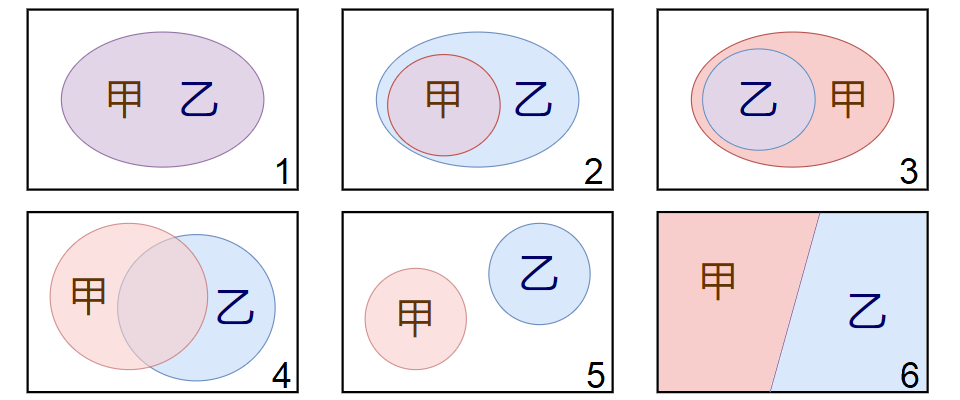
\includegraphics[width=0.75\textwidth]{tu/概念的关系1.png}
    \captionsetup{justification=centering}
    \caption*{1.\texttt{等同关系},2.\texttt{从属关系},3.\texttt{包含关系},\\4.\texttt{交叉关系},5.\texttt{互斥关系},6.\texttt{矛盾关系}。}
\end{figure}

为了更好理解,我们可以用\textbf{叠圈图}直观理解集合的关系。

如下图,每个圈表示一个集合\footnote{也可以用其他形状的区域。},圈内的区域表示属于该集合的元素,圈外的区域表示不属于该集合的元素,也就是该集合(关于全集的)补集。
两个圈重叠的部分就表示同时属于两者的元素的集合,也就是两个集合的交集。而两个圈各自的部分加上重叠的部分,
就是至少属于其中之一的元素的集合,也就是两个集合的并集。

叠圈图可以让我们直接看到集合之间的关系。可以看到,用集合来解释概念,方便得多。

\begin{xt}\label{xt:2-0-20}
    \mbox{} \\ 
    \indent 1. 请用集合解释概念的属加种差定义方法。\\
    \indent 2. 用叠圈图表示“偶数”、“$3$的倍数”、“自然数”之间的关系。\\
    \indent 3. 三个集合$A,B,C$都是集合$\{1,2,3,4,5,6\}$的子集,它们都不是空集,而且构成集合$\{1,2,3,4,5,6\}$的分划。\\
    \indent 3.1. 请写出一个符合条件的$A,B,C$的例子。\\
    \indent 3.2. 符合条件的$A,B,C$一共有几种?
\end{xt}

\section{判断和集合}
理解了概念和集合的关系,我们可以用集合的概念来重新看待判断和命题。

简单的性质判断,只涉及一个概念和一个性质。在对应的命题里,概念是主语,性质是谓语。
我们把主语的概念记为$A$,把谓语的性质记为$b$,那么简单的性质判断可以写成:
$$ A \,\,\mbox{是} \,\,b. $$
如果把$a$看成集合,把用$B$表示所有具有性质$b$的东西的集合。那么,性质判断“$A$是$b$”就是说:
$$A \subseteq B$$
所以,简单的性质判断,就是描述概念的从属关系,也就是集合的子集关系。
判断为真,就是说$A \subseteq B$成立;判断为假,就是说$A \subseteq B$不成立。

\begin{wrapfigure}[5]{r}{0.26\textwidth} %this figure will be at the right
    \vspace{-32pt}
    \flushright
    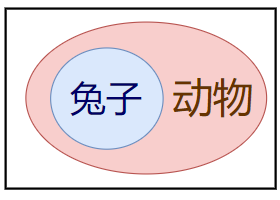
\includegraphics[width=0.24\textwidth]{tu/判断和集合1.png}
    \caption*{\texttt{命题:兔子是动物。}}
\end{wrapfigure}

如果判断的概念$A$是单独概念,那么它对应的子集只有一个元素。我们把这种只含有一个元素的集合称为\textbf{单元集}。

如果把$A$的元素记为$a$,那么$A = \{a\}$。$\{a\} \subseteq B$实际上就是说$a\in B$。

也就是说,判断的概念$A$是单独概念时,我们实际在判断概念是否属于有某个性质的集合。

我们可以给判断的概念$A$加上全称和有称,比如“所有$A$都是$b$”。“所有”的意思是,
概念$A$的范围里所有的元素,都是$b$。于是,“所有”其实只是再次强调了子集关系。

在数学语言里,我们引进表示全称的符号:$\forall$。它读作“任一”、“任何”、“每个”。
全命题:“所有$A$都是$b$”可以记作“$\forall x \in A$,$x \in B$”。它的意思是“$A$中任一元素都是$B$的元素”。
也就是说,$A$是$B$的子集。

如果我们说“有些$A$是$b$”,我们要表达的意思是,$A$的元素里,有些元素是$b$。这些元素构成$A$的子集,但不一定是$A$。
所以,有命题其实表示$A$和$B$相交,交集不是空集。

\begin{figure}[h]
    \vspace{4pt}
    \centering
    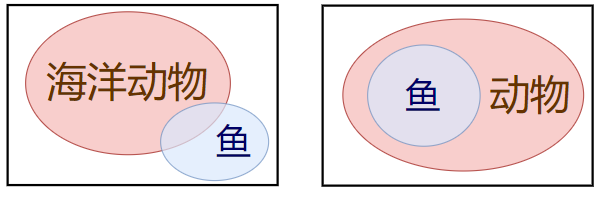
\includegraphics[width=0.5\textwidth]{tu/判断和集合2.png}
    \captionsetup{justification=centering}
    \caption*{\texttt{左:有些鱼是海洋动物,右:所有的鱼都是动物。}}
\end{figure}

在数学语言里,我们引进表示有称的符号:$\exists$。它读作“存在”,“有”,“至少有一个”。
有命题“有些$A$是$b$”可以记作“$\exists x \in A$,$x \in B$”。它的意思是“$A$中至少有一元素是$B$的元素”。
也就是说,$A$和$B$的交集不是空集。

举例来说,“所有偶数都是自然数”可以写作“$\forall x \in \{\mbox{偶数}\}$,$x \in \{\mbox{自然数}\}$”,
换句话说,偶数集是自然数集的子集。
“有些偶数是$3$的倍数”可以写作“$\exists x \in \{\mbox{偶数}\}$,$x \in \{3\mbox{的倍数}\}$”,换句话说,
偶数集和$3$的倍数的集合相交,交集不是空集。

\begin{et}
    用代数的方法,表示加法和乘法的交换律、结合律。
\end{et}

\begin{so}
    加法的交换律:任意两个数相加,交换次序,和不变。把两个数用$a$、$b$表示,加法交换律可以表示成:
    $$ \forall \,\, a, b, \quad a + b = b + a. $$
    
    加法的结合律:任意三个数相加,先把前两个数相加,或者先把后两个数相加,和不变。把三个数用$a$、$b$、$c$表示,加法结合律可以表示成:
    $$ \forall \,\, a, b, c, \quad (a + b) + c = a + (b + c). $$
    
    乘法的交换律:任意两个数相乘,交换次序,积不变。把两个数用$a$、$b$表示,乘法交换律可以表示成:
    $$ \forall \,\, a, b, \quad a \times b = b \times a. $$
    
    乘法的结合律:任意三个数相乘,先把前两个数相乘,或者先把后两个数相乘,积不变。把三个数用$a$、$b$、$c$表示,乘法结合律可以表示成:
    $$ \forall \,\, a, b, c, \quad (a \times b) \times c = a \times (b \times c). $$
\end{so}

复合判断,也可以用集合的方式表达。

联言判断是多个判断的全判断。考虑这样的联言判断:$A$不仅是$b$,也是$c$。
它表达的意思是,$A$不仅包含于性质$b$对应的集合$B$,也包含于性质$c$对应的集合$C$。
$A$的元素同时在$B$、$C$中。换句话说,$A$是$B$、$C$的交集的子集。

一般来说,考虑关于概念$A$的联言判断,它表达的是$A$包含于多个性质对应的集合的交集。
如果把这些性质的集合记为$I$,把每个性质对应的集合记为$B_i$,那么联言判断就是说,
$A$包含于它们的交集,记为:
$$ A \subseteq \bigcap_{i\in I} B_i. $$

或言判断是多个判断的有判断。考虑这样的或言判断:$A$也许$b$,也许$c$。
它表达的意思是,$A$可能包含于性质$b$对应的集合$B$,也可能包含于性质$c$对应的集合$C$。
$A$的元素至少在$B$、$C$中的一个里。换句话说,$A$是$B$、$C$的并集的子集。

一般来说,考虑关于概念$A$的或言判断,它表达的是$A$包含于多个性质对应的集合的并集。
如果把这些性质的集合记为$I$,把每个性质对应的集合记为$B_i$,那么或言判断就是说,
$A$包含于它们的交集,记为:
$$ A \subseteq \bigcup_{i\in I} B_i. $$

\begin{wrapfigure}{r}{0.42\textwidth} %this figure will be at the right
    \vspace{-28pt}
    \flushright
    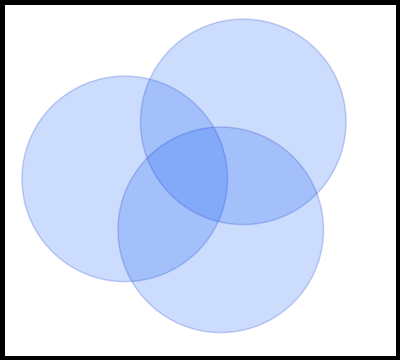
\includegraphics[width=0.4\textwidth]{tu/叠圈图1.png}
\end{wrapfigure}

右图中,每个圈代表一个分支判断对应的集合。联言判断对应着所有圈交叠的区域(颜色最深的部分),而或言判断对应着所有蓝色的区域的总和。

\begin{sk}\label{sk:2-1-1}
     有个理发师,坚持只给那些不给自己理发的人理发。那么,他是否该给自己理发呢?
\end{sk}

\begin{xt}\label{xt:2-1-1}
    \mbox{} \\
    \indent 1. 用代数的方法,表示乘法对加法的分配律。\\
    \indent 2. 用代数的方法,表示乘方的运算法则。\\
    \indent 3. 考虑假言判断:如果$A$是$b$,那么$A$是$c$。设性质$b$、$c$对应的集合是$B$、$C$,集合$A$、$B$、$C$之间有什么关系?\\
    \indent 4. 从集合的角度,解释这句话:“如果全部$A$都是$b$,那么有些$A$是$b$”。
\end{xt}

\section{映射}
我们用\textbf{映射}表示事物之间的对应关系。把一个事物对应到另一个事物,可以理解为事物的变换或对事物进行操作。
因此映射也叫做\textbf{变换}或\textbf{操作}。把数量对应到数量的映射,叫做\textbf{函数}。

\begin{ex}\label{ex:2-2-0}
    \mbox{} \\ 
    \indent 1. 把现有《道德经》各个版本和它的字数对应起来,就是一个映射:
    $$
    \begin{array}{lll}
        \mbox{王弼《老子道德经注》(通行本)} &\longrightarrow &\quad 5162\mbox{字} \\
        \mbox{河上公《道德经章句》} &\longrightarrow &\quad 5201\mbox{字} \\ 
        \mbox{傅奕《道德经古本》} &\longrightarrow &\quad 5450\mbox{字} \\
        \mbox{马王堆帛书甲本} &\longrightarrow &\quad 5344\mbox{字} \\
        \mbox{马王堆帛书乙本} &\longrightarrow &\quad 5342\mbox{字} \\
        \mbox{郭店楚墓本} &\longrightarrow &\quad 2046\mbox{字}
    \end{array}
    $$
    \indent 2. 把事物对应到自己的映射叫做\textbf{恒等映射}或\textbf{等映射}。比如,把每个自然数对应到自己的映射就叫自然数集上的恒等映射,也叫恒等函数。任何非空集合上都有恒等映射。恒等映射的定义域和值域相同。\\
    \indent 3. 把事物对应到同一个对象的映射叫做\textbf{恒映射}或\textbf{常映射}。比如,把任意自然数对应到$0$的映射就是恒映射。
\end{ex}

我们把映射涉及的事物用两个集合记录:\textbf{出发集}和\textbf{到达集}。映射把出发集的一个元素对应到到达集的一个元素。
用变量$x$指代出发集的元素,$x$的取值在出发集里变化时,映射对应的元素也在到达集里变化,可以用变量$y$表示。
一般称$x$为\textbf{自变量},$y$为\textbf{应变量}。出发集和到达集都是数集的时候,映射就叫做函数。

需要强调的是,映射可以把多个元素对应到同一个元素,但不会把一个元素对应到多个元素。

% 来自 https://commons.wikimedia.org/wiki/File:Function_color_example_3.svg
\begin{figure}[h]
    \vspace{4pt}
    \centering
    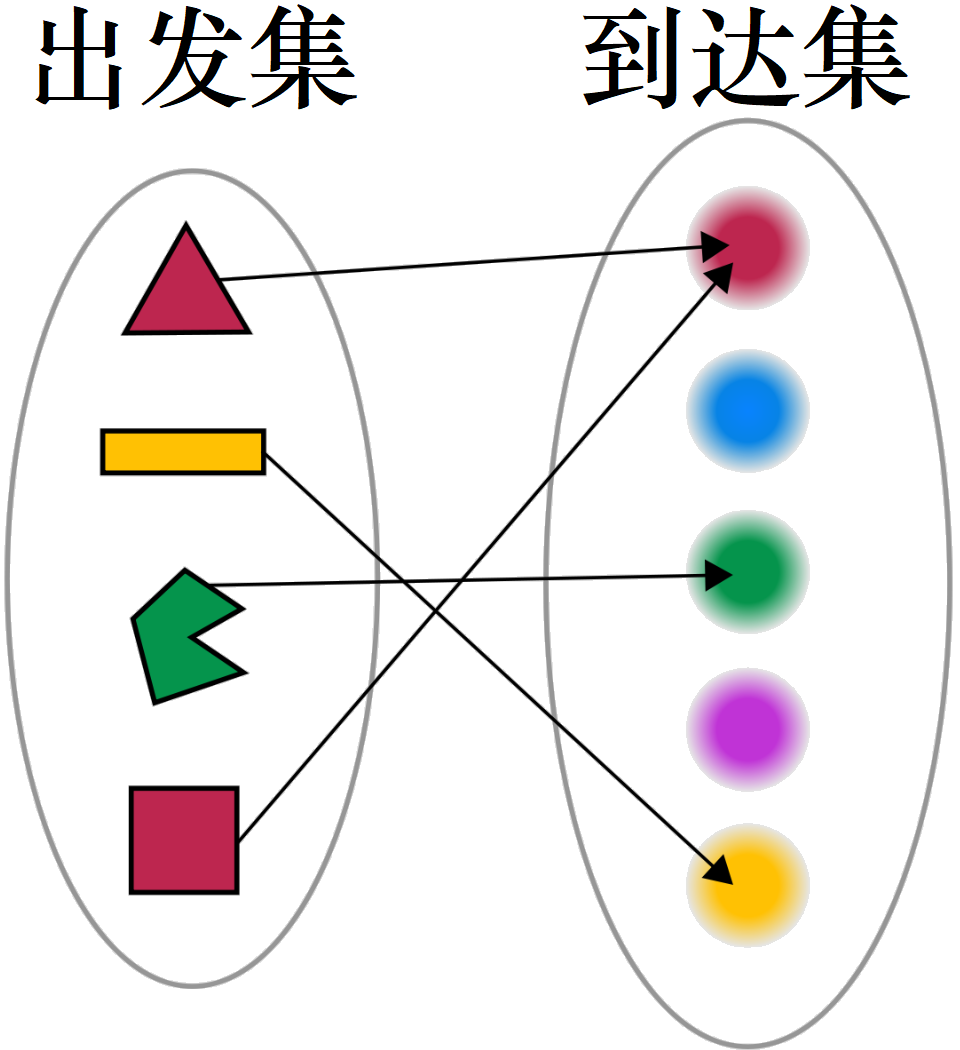
\includegraphics[width=0.5\textwidth]{tu/映射1.png}
    \caption*{\texttt{映射把图形对应到它的颜色}}
\end{figure}

如果把映射记作$f$,那么可以用$y = f(x)$或$f:x\mapsto y$表达“映射把出发集的元素和到达集的元素对应起来”这件事。
对出发集的元素$x$来说,如果映射$f$把它和到达集的元素$y$对应起来,就说$y$是$x$(经过$f$映射)的\textbf{值},记作$f(x) = y$。

出发集中,某个映射涉及的元素集合称为映射的\textbf{定义域};
到达集里,某个映射涉及的元素集合则称为映射的\textbf{值域}。定义域是出发集的子集,值域是到达集的子集。

举例来说,映射$f$的定义域是$\{1,2,3,4,5\}$,它把$1,2,3,4,5$分别对应到$6,7,8,7,6$。
那么它的值域是$\{6,7,8\}$。具体来说,$f(2) = 7$,$f(3) = 8$。

考虑映射$f$的定义域的子集$S$。$S$中元素经过$f$映射的值,构成值域的子集。
我们把它叫做$S$(关于$f$)的\textbf{像集},简称$S$的\textbf{像},记作$f(S)$。

反之,考虑映射$f$的值域的子集$T$。$T$中元素总是$f$的定义域中元素的值。
我们把$f$的定义域里值属于$T$的元素集合起来。这个集合叫做$T$关于$f$的\textbf{原像}。

举例来说,映射$f$的定义域是$\{1,2,3,4,5\}$,它把$1,2,3,4,5$分别对应到$6,7,8,7,6$。
那么,集合$\{1,2,3,4\}$的像集是$\{6,7,8\}$;集合$\{1,2\}$的像集是$\{6,7\}$。
集合$\{7,8\}$的原像是$\{2,3,4\}$;集合$\{6,8\}$的原像是$\{1,3,5\}$。

我们约定,空集的像集是空集,空集的原像是空集。

每个一元式都可以用来定义映射。比如,设定定义域是自然数集$\mathbb{N}$后,
代数式$4-0.3x+9x^2+\frac{(1-x+2.69x^4)}{0.5x-1.385}$就可以定义映射:
$$ \forall x\in\mathbb{N}, \quad x \mapsto 4-0.3x+9x^2+\frac{(1-x+2.69x^4)}{0.5x-1.385}. $$
如果把定义域设成另一个集合,比如$\{1,2,3\}$或全体偶数,就定义了另一个映射。

我们知道,每个概念都对应某种集合。如果我们把这个集合作为定义域或者出发集,那么,
确定了定义域后,每个含有变量的简单性质判断就可以定义一个映射。

比如,考虑这样一个命题:“$\{1,2,5,6\}$中的任何数$n$都能被$5$整除”。
我们可以看到,定义域是$\{1,2,5,6\}$,而“$n$能被$5$整除”就可以定义以下的映射:
$$ \forall n\in \{1,2,5,6\} , \quad n \mapsto n\,\mbox{能被}\,5\,\mbox{整除。} $$
这个映射从简单判断的主语出发。主语的概念对应集合$\{1,2,5,6\}$。

对集合中每个单独的元素$n$,
“$n$能被$5$整除”这个判断要么是真的,要么是假的。因此,如何我们考虑集合$\{\mbox{真}, \mbox{假}\}$,
那么这个集合就是上面的映射的到达集,因为对每个$n$来说,“$n$能被$5$整除”这个判断要么是真的,要么是假的。
而它的值域就是集合$\{\mbox{真}, \mbox{假}\}$的子集。

“真”、“假”就是命题的真值,所以我们一般把这个集合称为\textbf{真值集}或者\textbf{二元集}。
很多时候,我们也会用$0$表示“假”,$1$表示“真”\footnote{也有的时候会反过来。}。

\begin{sk}\label{sk:2-2-0}
    \mbox{} \\
    \indent 1. 全判断$\forall x \in A, \, P(x)$和映射$x \mapsto P(x)$之间存在什么关系?\\
\end{sk}

\begin{xt}\label{xt:2-2-0}
    \mbox{} \\
    \indent 1. 映射$f$的定义域是$\{1,2,3\}$,值域是$\{4,5\}$。\\
    \indent 1.1. 写出一个满足条件的映射$f$。\\
    \indent 1.2. 你能写出几个满足条件的映射$f$?\\
    \indent 2. 判断以下说法是否正确。\\
    \indent 2.1. 到达集中的元素,总是映射的结果。\\
    \indent 2.2. 出发集中的元素经过映射的值,总在映射的值域中。\\
    \indent 2.3. 映射的定义域的元素构成的集合,其像集的原像总是自己。\\
    \indent 2.4. 映射的值域的元素构成的集合,其原像的像集总是自己。\\
    \indent 3. 考虑以下映射和集合,给出相应的像集或原像。\\
    \indent 3.1. 映射$f$把正整数对应到它的$3$倍数。比如:$f(1) = 3$,$f(2) = 6$,等等。求集合$\{21, 39, 87\}$的像集和原像。\\
    \indent 3.2. 映射$g$把月份对应到它的天数(不考虑闰年)。比如一月的值是$31$,二月的值是$28$,等等。求集合$\{30\}$的原像。\\
    \indent 3.3. 映射$h$把汉字对应到它的笔画数。比如“数”的值是$13$,“学”的值是$8$,等等。设集合$S$是$\{1,2\}$的原像,请写出它的十个元素。 % 一二七八九 十人入丁乃 儿了几刀刁 力匕卜厂又
\end{xt}

\chapter{有理数的运算}
我们已经学过自然数和分数的运算。两个自然数可以做加法、减法和乘法,任两个分数可以做加法、减法、乘法和(不为零的)除法。
把自然数、分数扩展到有理数后,两个有理数可以做加法、减法、乘法和不为零的除法。

有理数的运算和自然数、分数相比,多了与负数有关的运算。为了讨论方便,我们首先介绍一个表示负数的方法:
每个负数都能表示成$-a$的形式,其中$a$是它的相反数,是一个正数。

\section{有理数的加减法}
我们先来看与负数有关的加减法。按照负数的定义,任何负数$-a = 0 - a$。
所以,一个数加上一个负数,就等于减去它的相反数:
$$ b + (-a) = b + (0 - a) = (b + 0) - a = b - a.$$
换句话说,减去一个正数,就等于加上它的相反数。另一方面:
$$ b - (-a) = b + a - a - (-a) = b + a + (-a) - (-a) = b + a.$$
换句话说,减去一个负数,也等于加上它的相反数。

两者可以用同一句话描述:\textbf{减去一个数,等于加上它的相反数。}

\begin{center}
    \begin{tikzpicture}[>=latex]
 \node at (0,0) {$ b-a=b+(-a)$}  ;
 \draw[draw=red,<->] (-1.08,.3)--(-1.08,1)--node[above]{减法化加法}(.38,1)--(.38,.3);
 \draw[draw=blue,<->] (-.69,-.3)--(-.69,-1)--node[below]{换成相反数}(1.12,-1)--(1.12,-.3);
    \end{tikzpicture}
\end{center}

于是,有理数的减法总可以转化为有理数的加法。

\begin{ex}
    \indent 1. 计算:
    $$
    \begin{array}{ll}
        (1). \quad 3.4 - (-2.1) \quad & \quad (2). \quad 2.8 - (-5) \\
        (3). \quad 9.1 - (-4.6) \quad & \quad (4). \quad 1.2 - (-4.4) 
    \end{array}
    $$
    \indent 2. 把以下减法改为加法:
    $$
    \begin{array}{ll}
        (1). \quad 3.4 - 2.1 \quad & \quad (2). \quad 2.8 - 5 \\
        (3). \quad -9.1 - (-4.6) \quad & \quad (4). \quad -1.2 - (-4.4) 
    \end{array}
    $$

\end{ex}
\begin{so}
    \mbox{}\\
    \indent 1. \\
    \indent $(1). \quad 3.4 - (-2.1) = 3.4 + 2.1 = 5.5$ \\
    \indent $(2). \quad 2.8 - (-5) = 2.8 + 5 = 7.8$ \\
    \indent $(3). \quad 9.1 - (-4.6) = 9.1 + 4.6 = 13.7$ \\
    \indent $(4). \quad 1.2 - (-4.4) = 1.2 + 4.4 = 5.6$ \\
    \indent 2. \\
    \indent $(1). \quad 3.4 - 2.1 = 3.4 + (-2.1)$ \\
    \indent $(2). \quad 2.8 - 5 = 2.8 + (-5)$ \\
    \indent $(3). \quad -9.1 - (-4.6) = -9.1 + 4.6$ \\
    \indent $(4). \quad -1.2 - (-4.4) = -1.2 + 4.4$ 
\end{so}

再来看两个有理数的加法。我们要计算:
$$ a + b $$

如果两者都是正数,就是我们熟悉的分数加法。

如果两者都是负数,那么$-a$、$-b$都是正数:
$$ 0 = 0 + 0 = (a +(-a)) + (b + (-b)) = a + b + \left((-a) + (-b)\right).$$
因此,和是$(-a) + (-b)$的相反数。

如果$a$、$b$一正一负,不妨设$a$正$b$负\footnote{如果$a$负$b$正,根据加法交换律,可以转化成$a$正$b$负的情形。},于是$-b$是正数。
$$ a + b = a - (-b)$$
式子中$a$和$-b$都是正数。如果$a > -b$,那么$a - (-b)$是正数。如果$a < (-b)$,那么$a - (-b)$是负数。而由于:
$$ 0 = 0 + 0 = a - a + (-b) - (-b) = \left(a - (-b)\right) + \left((-b) - a\right),$$
因此$a - (-b)$和$(-b) - a$互为相反数。也就是说,$a + b$是正数$(-b) - a$的相反数。

看得出,上面讨论中$a$和$-b$的大小关系很重要。为了方便总结,我们引进\textbf{绝对值}的概念:
\begin{df}\label{df:3-0-0}
    正数的\textbf{绝对值}是它自身,负数的绝对值是它的相反数。$0$的绝对值是$0$。
\end{df}
按照这个定义,可以把前面讨论的结果简化:

如果两个有理数同为正数(负数),那么它们的和也是正数(负数),绝对值是它们绝对值的和。
如果两个有理数一正一负,那么它们的和的正负与绝对值较大者的正负一致,
和的绝对值是绝对值较大者减去绝对值较小者的差。

总结两个有理数的加减法:
\begin{center}
    \fbox{
        \shortstack[l]{
            1. 将减法转为加法。\\
            2. 任何数与$0$相加都得到自身。\\
            3. 计算两个数的绝对值。\\
            4. 如果两个数同正负,取绝对值的和,加上对应的正负号。\\
            5. 如果两个数一正一负,用较大的绝对值减去较小的绝对值,\\
            加上绝对值较大的数的正负号。
        }
    }
\end{center}

\begin{ex}
    计算:
    $$
    \begin{array}{lll}
        (1). \quad 3.4 - (-2.1) \quad & \quad (2). \quad 2.8 - 5 \quad & \quad (3). \quad -7 + 2.3 \\
        (4). \quad -9.1 + (-4.6) \quad & \quad (5). \quad -1.2 + 4.4 \quad & \quad (6). \quad -0.9 - 3.4
    \end{array}
    $$
\end{ex}
\begin{so}
    \mbox{}\\
    \indent $(1). \quad 3.4 - (-2.1) = 3.4 + 2.1 = 5.5$ \\
    \indent $(2). \quad 2.8 - 5 = 2.8 + (-5) = -(5 - 2.8) = -2.2$ \\
    \indent $(3). \quad -7 + 2.3 = -(7 - 2.3) = -4.7$ \\
    \indent $(4). \quad -9.1 + (-4.6) = -(9.1 + 4.6) = -13.7$ \\
    \indent $(5). \quad -1.2 + 4.4 = 4.4 - 1.2 = 3.2$ \\
    \indent $(6). \quad -0.9 - 3.4 = -0.9 + (-3.4) = -(0.9 + 3.4) = -4.3 $ 
\end{so}

\begin{xt}\label{xt:3-0-0}
    算一算:\\
    \indent 1. $2.56 - (-1.9)$,$(-4) + 3.29$,$10.8 + (-42.15).$ \\
    \indent 2. $-59.76 + 40.3$,$-2.8 - 6.6$,$-5.09 - (-2.9).$ \\
    \indent 3. $-1.76 -(-5.21) - 1.874$,$3.202 - (-1.94) - 1.57$,$2 + (-9.18) - (20.354).$ \\
    \indent 4. $3 - 2 - (-8) + (-2.2)$,$-8.1 - ((-1.6) - 1.96 + (-3.9 + 1.203)).$
\end{xt}

\section{有理数的乘除法}
讨论有理数的乘除法,可以从最简单的情况开始:$(-1) \times 1$和$(-1) \times (-1)$。按照定义,
$$0 = 0 \times 1 = (-1 + 1) \times 1 = (- 1) \times 1 + 1 \times 1 = (-1) \times 1 + 1.$$
于是
$$ (-1) \times 1 = 0 - 1 = -1.$$
同理,$(-1) \times 0 = 0$。
根据乘法交换律,$1 \times (-1) = -1$,$0 \times (-1) = 0$。

最后:
\begin{align*}
    0 = 0 \times (-1) &= (- 1 + 1) \times (-1)  \\
    &= (-1) \times (-1) + 1 \times (-1)  \\
    &= (-1) \times (-1) - 1. 
\end{align*}
于是$(-1) \times (-1) = 1.$

所以,$-1$的乘法性质可以归纳为“负零得零,负正得负,负负得正”。

同理,把乘数换成一般的数,也有:
$$(-1) \times a =  0 - a = -a, \quad (-1) \times (-a) = 0 - (-1) \times a = a.$$
也就是说,一个数乘以$-1$,总得到它的相反数。

从绝对值的角度来看,任何正数都等于它的绝对值,任何负数都等于它的绝对值乘以$-1$。
换句话说,在乘法中,任何有理数都可以分成两部分考虑:绝对值和正负号。

因此,两个有理数$a$、$b$相乘,可以分别把两部分相乘。比如:
$$ (-3.3) \times 6 = (-1) \times 3.3 \times (+1) \times 6 = ((-1) \times (+1)) \times (3.3 \times 6).$$
其中$3.3$、$6$分别是乘数和被乘数的绝对值,$-1$和$+1$是它们的正负号。

两个有理数的乘积,是两者绝对值的乘积,乘以两者正负号的乘积。绝对值的乘积总是正数,
正负号的乘积总是$\pm 1$。因此,两个有理数的乘积,绝对值是两者绝对值的乘积,正负号是两者正负号的乘积。
具体来说,看$-1$的个数,就可以确定乘积的正负了。
如果正负号都是正数,那么不需要考虑$-1$的问题。如果两者一正一负,那么乘积是负数,
如果正负号都是负数,“负负得正”,于是乘积是正数。

如果乘数或被乘数是$0$,结果是$0$。

除法是乘法的逆运算。除以一个正有理数$a$,等于乘以它的倒数:$\frac{1}{a}$。
我们只需要把涉及负数的除法也转为乘法即可。

除数是负有理数$-a$的时候,我们首先找到$b \div (-a)$的商,也就是使得$c \times (-a) = b$的数$c$。
根据前面对乘法的推导,
$$ b \times (-1) \times \frac{1}{a} = c \times (-a) \times (-1) \times \frac{1}{a} = c \times a \times \frac{1}{a} = c$$
或者说
$$c = b\times \left((-1) \times \frac{1}{a}\right) = b\times \left(-\frac{1}{a}\right) .$$
即
$$b \div (-a) = b\times \left(-\frac{1}{a}\right). $$
最后,我们说明$-\frac{1}{a}$是$-a$的倒数:
\begin{align*}
    (-a) \times \left(-\frac{1}{a}\right) &= a \times (-1) \times (-1) \times \frac{1}{a} \\
    &= (-1)\times (-1) \times a \times \frac{1}{a} \\
    &= 1 \times 1 = 1.
\end{align*}

所以,无论除数是正有理数还是负有理数,\textbf{除以一个数,等于乘以它的倒数。}

\begin{center}
    \begin{tikzpicture}[>=latex]
 \node at (0,0) {$\displaystyle b\div a=b\times \frac{1}{a}$}  ;
 \draw[draw=red,<->] (-.8,.3)--(-.8,1)--node[above]{除法化乘法}(.66,1)--(.66,.3);
 \draw[draw=blue,<->] (-.42,-.3)--(-.42,-1)--node[below]{换成倒数}(1.1,-1)--(1.1,-.6);
    \end{tikzpicture}
\end{center}

于是,有理数的除法总可以转化为有理数的乘法。

综上所述,可以这样总结有理数的乘除法:
\begin{center}
    \fbox{
        \shortstack[l]{
            1. 将除法转为乘法。\\
            2. 任何数与$0$相乘都得到$0$。\\
            3. 计算两个数的绝对值。\\
            4. 如果两个数同正负,取绝对值的乘积。\\
            5. 如果两个数一正一负,取绝对值乘积的相反数。
        }
    }
\end{center}
\begin{ex}
    计算:
    $$
    \begin{array}{lll}
        (1). \quad 3.3 \times (-5) \quad & \quad (2). \quad -\frac{3}{7} \times (- \frac{5}{6}) \quad & \quad (3). \quad (-2.4) \times \frac{1}{6} \\
        (4). \quad 4.8 \div (-1.6) \quad & \quad (5). \quad -\frac{3}{7} \div (- \frac{5}{14}) \quad & \quad (6). \quad (-2.8) \div \frac{2}{3}
    \end{array}
    $$
\end{ex}
\begin{so}
    \mbox{}\\
    \indent $(1). \quad 3.3 \times (-5) = -(3.3 \times 5) = -16.5$ \\
    \indent $(2). \quad -\frac{3}{7} \times (- \frac{5}{6}) = \frac{3}{7} \times \frac{5}{6} = \frac{5}{14}$ \\
    \indent $(3). \quad (-2.4) \times \frac{1}{6} = -(2.4 \times \frac{1}{6}) = -0.4$ \\
    \indent $(4). \quad 4.8 \div (-1.6) =  4.8 \times (-\frac{5}{8}) = -(4.8 \times \frac{5}{8}) = -3$ \\
    \indent $(5). \quad -\frac{3}{7} \div (- \frac{5}{14}) = -\frac{3}{7} \times (- \frac{14}{5}) = \frac{3}{7} \times \frac{14}{5} = 1.2$ \\
    \indent $(6). \quad (-2.8) \div \frac{2}{3} = (-2.8) \times \frac{3}{2} = -(2.8 \times \frac{3}{2}) = -4.2 $ 
\end{so}

\begin{xt}\label{xt:3-1-0}
    \mbox{}\\
    \indent 算一算:\\
    \indent $4.51 \times (-2.2)$,$(-1.2) \times (-3.9)$,$(-1.8)\times 0.8.$ \\
    \indent $1.98 \div (-0.3)$,$-2.8 \div (-0.7)$,$5.2 \div (3 \div (-1.5))$, $(-3) \div (0.5 \times (-2.4)).$ \\
    \indent 思考:\\
    \indent 1. 为什么“任何数与$0$相加都得到自身”?\\
    \indent 2. 为什么“任何数与$0$相乘都得到$0$”?\\
    \indent 3. 为什么说“涉及负数的乘法也满足交换律和分配律”?
\end{xt}

\section{数轴}
为了直观表示有理数,我们引入\textbf{数轴}的概念。

从左往右画一条直线,在直线上取一点表示$0$,称为\textbf{原点}。
选择适当长度作为\textbf{单位长度},规定右边是\textbf{正方向},
往右移动一个单位长度就是“$+1$”。

那么,从原点出发往右移动,每移动一个单位长度就是“$+1$”。因此,每隔单位长度取一个点,就可以表示出$1,2,3\cdots$。
相对的,往左移动一个单位长度就是“$-1$”,类似可以表示出$-1,-2,-3\cdots$。这就是数轴。

数轴上的点,越往右就越大,越往左就越小。正数都在$0$右边,负数都在$0$左边。
两个数比较大小,可以在数轴上找到对应的点:靠右的比较大,靠左的比较小。

数轴上的相反数:$3$是从原点往右移动$3$个单位长度到达的点,而$-3$是从原点往左移动$3$个单位长度到达的点。
如果先往右移动$3$个单位长度,再往左移动$3$个单位长度,就会回到原点。
一般来说,在数轴上先往右再往左(或先往左再往右)走一样多的单位长度,
最终自然就回到原点。这说明任何数加上自己的相反数,都得到$0$。

\begin{sk}\label{sk:3-2-0}
    有理数在数轴上吗?怎么在数轴上找到一个有理数?
\end{sk}

\chapter{代数式的运算}
代数式是含有变量的算式。代数式的运算和数式并没有区别。毕竟,代数式里的变量只是用来
代替数的。对代数式做运算,使用和数式运算一样的规则:加法结合律、乘法结合律、加法交换律、
乘法交换律,以及乘法对加法的分配律。

\section{整式的运算}

与整式有关的计算,一个常见的目标是把式子\textbf{展开},也就是把几个整式的乘积转成一个整式:单项式或多项式。
展开整式,可以按照以下步骤操作:
\begin{enumerate}
    \item 用分配律把整式乘积转为整式中各项的乘积之和。
    \item 合并同类项(用到结合律和交换律)。
\end{enumerate}
\begin{ex}\label{ex:5-0-0}
    计算:\\
    1. 展开并化简$(a + b)(a - b)$\\
    \textbf{解}:
    \begin{align*}
        (a + b)(a - b) &= a\cdot (a - b) + b\cdot (a - b) \tag{分配律展开} \\
        &= a\cdot a - a\cdot b + b\cdot a - b\cdot b \\
        &= a^2 + (-1 + 1)ab - b^2  \tag{合并同类项}\\
        &= a^2 + 0ab - b^2 \\
        &= a^2 - b^2 
    \end{align*}
    2. 展开并化简$(a^2 + ab - b^2)(a - b)$\\
    \textbf{解}:
    \begin{align*}
        &\quad\, (a^2 + ab - b^2)(a - b) \\
        &= a^2\cdot (a - b) + ab\cdot (a - b) + (- b^2)\cdot (a - b) \tag{分配律展开} \\
        &= a^2\cdot a - a^2\cdot b + ab\cdot a - ab\cdot b + (- b^2)\cdot a + (-b^2) \cdot (-b)  \\
        &= a^2\cdot a - a^2\cdot b + a^2b - ab^2 - b^2\cdot a + b^2 \cdot b  \\
        &= a^3 + (-1 + 1)a^2b + (-1 - 1)ab^2 + b^3 \tag{合并同类项}\\
        &= a^3 + 0a^2b - 2ab^2 + b^3 \\
        &= a^3 - 2ab^2 + b^3 
    \end{align*}
\end{ex}

在第一个例子中,我们首先把$a - b$看成一个整体,把$a + b$看成两项相加。
使用分配律,就把$(a + b)(a - b)$转为$a\cdot (a - b)$与$b\cdot (a - b)$的和。
接下来,我们把$a - b$看成两项相减,再次使用分配律,就把$(a + b)(a - b)$完全转成若干项的和:
$$ a\cdot a - a\cdot b + b\cdot a - b\cdot b$$
接着,我们合并同类项。使用交换律,可以知道$ab = ba$,所以这两项是同类项,可以合并。合并后,
系数是$-1 + 1 = 0$,所以这$ab$项被消去了。剩下的两项无法合并同类项了。于是我们最后得到:
$$(a + b)(a - b) = a^2 - b^2. $$

第二个例子中的计算步骤也是如此。需要注意的是,展开$(- b^2)\cdot (a - b)$这样带有多个减号(负号)的式子时,
要仔细处理正负号。为了防止出错,可以先将容易出错的减法转为加法。比如,计算$ab - b(a-c)$时,可以把它化为:
$ab+(-b)\cdot(a + (-c))$。使用分配律展开各项之后,再用“负正得负,负负得正”的法则,消去负号,化简各项。
比如,展开$ab - b(a-c)$:
\begin{align*}
    ab - b(a-c) &= ab+(-b)\cdot(a + (-c)) \tag{减法化加法}\\
    &= ab + (-b)\cdot a + (-b) \cdot (-c) \tag{分配律展开} \\
    &= ab - ba + bc \tag{消去负号}\\
    &= bc.
\end{align*}

另一种常见的代数式计算叫做\textbf{变量代换}。我们知道,变量是用来代替数的。其实,变量也可以用来代替变量。
用变量代替变量,可以变化代数式的形式,很多时候,可以帮助我们更好地理解事物间的关系。

举例来说,我们想展开$(a - 2b + 1)(a - 2b - 1)$,除了像上面的例子一样直接使用分配律然后合并同类项,还有什么别的方法吗?

我们可以观察到,这个式子是两个整式的乘积,第一个是$a - 2b$与$1$的和,第二个是$a - 2b$与$1$的差。
于是,我们可以把$a - 2b$看成一个整体,把$1$看成一个整体。我们用变量$x$代替$a - 2b$,$y$代替$1$,
那么原式就变成了$(x + y)(x - y)$,于是等于$x^2 - y^2$。

我们再把$x$和$y$代替的变量和数代回去,就得到原式等于$(a - 2b)^2 - 1^2$。$1^2 = 1$,
所以我们现在只需要展开$(a - 2b)^2$了。展开$(a - 2b)^2$:
\begin{align*}
    (a - 2b)^2 &= (a - 2b)(a - 2b)  \\
    &= (a - 2b)\cdot a - (a - 2b) \cdot 2b  \\
    &= a^2 -2b\cdot a -a\cdot 2b + 2b\cdot 2b  \\
    &= a^2 + (-2 -2) ab + 4b^2  \\
    &= a^2 - 4ab + 4b^2 
\end{align*}
因此,
$$ (a - 2b + 1)(a - 2b - 1) = (a - 2b)^2 - 1 = a^2 - 4ab + 4b^2 - 1.$$

数学中常用的整式等式:\\
\indent $1. \quad (a + b)^2 = a^2 + b^2 + 2ab $ \\
\indent $2. \quad (a - b)^2 = a^2 + b^2 - 2ab $ \\
\indent $3. \quad (a + b)(a - b) = a^2 - b^2 $ \\
\indent $4. \quad (a + b)^3 = a^3 + 3a^2b + 3ab^2 + b^3 $ \\
\indent $5. \quad (a - b)^3 = a^3 - 3a^2b + 3ab^2 - b^3 $ \\
\indent $6. \quad a^3 + b^3 = (a^2 - ab + b^2)(a + b) $ \\
\indent $7. \quad a^3 - b^3 = (a^2 + ab + b^2)(a - b) $ \\
\indent $8. \quad (a + b + c)^2 = a^2 + b^2 + c^2 + 2ab + 2bc + 2ca $ \\
\indent $9. \quad (a + b)(a + c) = a(a + b + c) + bc $ \\
\indent $10. \quad (a + b)(b + c)(c + a) + abc = (a + b + c)(ab + bc + ca) $ \\
\indent $11.\quad  a^3+b^3+c^3 - 3abc = (a + b + c)(a^2+b^2+c^2-ab-bc-ca) $ 

\begin{xt}\label{xt:5-0-0}
    \mbox{}\\
    \indent 1. 展开并化简:\\
    \indent 1.1. $(4a + 2b - 1)(a - 3b + 1).$\\  % 4a^2 - 10ab - 6b^2 + 3a + 5b - 1
    \indent 1.2. $(a + b^2 - b - 2a^2)(a^2 - 2b^2 + a + b).$\\  % -2a^4 + 5a^2b^2 - 2b^4 -a^3 - 3a^2b - ab^2 + 3b^3 + a^2 - b^2
    \indent 2. 验证以下等式:\\
    \indent 2.1. $(a + b)^2 + (a - b)^2 = 2a^2+2b^2.$\\
    \indent 2.2. $a^4 + a^2 + 1 = (a^2+a+1)(a^2-a+1).$\\
    \indent 2.3. $3(a-b)(b-c)(c-a) = (a-b)^3+(b-c)^3+(c-a)^3$\\
    \indent 3. 求以下代数式中$x^3$的系数:\\
    \indent 3.1. $(x - 2)^5.$\\
    \indent 3.2. $(x^2 - x + 1)(x^3 - x^2 +2x - 1).$
\end{xt}

\section{分式的运算}

和分数一样,分式运算常见的目的有\textbf{约分}和\textbf{通分}。约分是把分子和分母中共有的式子消去,让分式更简洁。
无法继续约分的分式叫做既约分式。
通分是让几个分式的分母相同,以便相加。约分和通分的方法和分数相同。

\begin{ex}\label{ex:5-1-0}
    通分:\\
    1. $\frac{b+c}{a} + \frac{c+a}{b} + \frac{a+b}{c}$\\
    \textbf{解}:
    \begin{align*}
        \frac{b+c}{a} + \frac{c+a}{b} + \frac{a+b}{c} &= \frac{(b+c)bc+(a+c)ac+(a+b)ab}{abc} \\
        &= \frac{ a^2b+b^2c+c^2a + ab^2+bc^2+ca^2}{abc} 
    \end{align*}

    2. $\frac{a+2b}{a+b-1} - \frac{a+b+1}{a-b+1}$\\
    \textbf{解}:
    \begin{align*}
        \frac{a+2b}{a+b-1} - \frac{a+b+1}{a-b+1} &= \frac{(a+2b)(a-b+1) - (a+b+1)(a+b-1)}{(a+b-1)(a-b+1)} \\
        &=  \frac{a^2-ab+a+2ab-2b^2+2b - (a^2+2ab+b^2-1)}{(a+b-1)(a-b+1)}  \\
        &= \frac{-ab-3b^2+a+2b+1}{(a+b-1)(a-b+1)} 
    \end{align*}
\end{ex}

\begin{xt}\label{xt:5-1-0}
    \mbox{}\\
    \indent 1. 通分:\\
    \indent 1.2. $\frac{1}{a+b} + \frac{1}{2a-b}.$\\  % \frac{3a}{(a+b)(2a-b)}
    \indent 1.2. $\frac{a^2}{a+1} + \frac{a+1}{a-1}.$\\  % \frac{a^3 + 2a + 1}{(a-1)(a+1)}
    \indent 1.1. $\frac{a+b}{a+b+c} + \frac{c-a}{a+b-c}.$\\  % \frac{2a^2 + 3ab - ac + b^2 -2bc -c^2}{(a+b+c)(a+b-c)}
    \indent 2. 验证以下等式:\\
    \indent 2.1. $\frac{1}{a+b} + \frac{1}{a-b} = \frac{2a}{a^2-b^2}.$\\
    \indent 2.2. $\frac{a}{a+b} + \frac{b}{a-b} = \frac{a^2+b^2}{a^2-b^2}.$\\
    \indent 3. 求以下代数式中$x$的系数:\\
    \indent 3.1. $(x^2 - \frac{1}{x})^5.$\\  % -10
    \indent 3.2. $(x - x^2 - \frac{1}{x} + 1)(x^2 + x + 3 - \frac{2}{x}).$ % 5
\end{xt}

\chapter{从变量到方程(下)}

\section{一元一次方程}

\begin{ex}\label{ex:4-0-0}
    根据以下问题,设未知数并列出方程:\\
    $(1).$ 用一条$50$厘米长的丝带给一个正方形的盒子包装,捆好一周后,还有$26$厘米可以用于打结。盒子的边长是多少?\\
    $(2).$ 把一箱书分给某组学生阅读。如果每人分$3$本,则剩余$20$本;如果每人分$4$本,则还差$16$本。这个班有多少学生?
\end{ex}
\begin{so}
    \mbox{} \\
    $(1)$解:设盒子的边长是$x$厘米,列方程:
    $$ 4x + 26 = 50.$$
    $(2)$解:设这个班有$x$个学生,列方程:
    $$ 3x + 20 = 4x - 16.$$
\end{so}
以上的方程都有这样的性质:恰好含有一个变量来表示未知数,而且含有变量的项都是一次项。
这样的方程叫做\textbf{一元一次方程}。一元一次方程是由关于未知数的一元一次式构成的方程,它的一般形式是:$ax+b=cx+d$。
其中变量$x$是方程的未知数,$a,b,c,d$称为方程的系数。
实际的问题中,系数$a,b,c,d$是已知数,根据等式的基本性质,我们可以求出未知数$x$的值。

首先,我们把含有变量$x$的项移到等式一边,把常数项移到等式另一边。
利用等式的基本性质,我们将等式两边同时减去$b$,再同时减去$cx$,得到$ax-cx=d-b$。

$ax$和$cx$都是只含有$x$的一次项,它们之间只差一个系数,所以可以合并同类项:$ax - cx = (a - c)x$。

如果$a\neq c$,那么可以把等式两边同除以$a-c$,得到$x = \frac{d-b}{a-c}$。这就是方程的解。

如果$a = c$,那么我们得到$0 = d-b$。如果$b\neq d$,那么这个等式总是不成立的。
任何$x$的值都不能使等式成立。我们说方程无解。
如果$b = d$,那么我们得到$0 = 0$。这个等式总是成立的。任何$x$的值都能使等式成立。我们说方程有任意解。

使方程的等式成立的值是一个集合,称为它的\textbf{解集}。我们把上面的说法用集合的说法再表述一次:
方程无解,就是说方程的解集是空集。方程有任意解,就是说方程的解集是全集。方程有唯一解$x = \frac{d-b}{a-c}$,
就是说方程的解集就是$\{\frac{d-b}{a-c}\}$。
\begin{so}
    按这个方法,我们可以解以上两个问题中的方程:\\
    $(1)$解:设盒子的边长是$x$厘米,列方程:
    $$ 4x + 26 = 50.$$
    等式右边没有含变量的项,我们将等式两边同时减去$26$,得到:
    $$ 4x = 50 - 26.$$
    即:
    $$ 4x = 24. $$
    再将等式两边同时除以$4$,就得到解:$x=6$。\\
    答:盒子的边长是$6$厘米。\\
    $(2)$解:设这个班有$x$个学生,列方程:
    $$ 3x + 20 = 4x - 16.$$
    将等式两边同时减去$20$,再将等式两边同时减去$4x$,得到:
    $$ 3x - 4x = -20 - 16.$$
    左边合并同类项,右边计算减法,就得到:
    $$ -x = -36. $$
    再将等式两边同时除以$-1$,就得到解:$x = 36$。\\
    答:这个班有$36$个学生。
\end{so}
我们可以这样总结一元一次方程$ax+b=cx+d$的解:
\begin{center}
    \fbox{
        $ \left\{ \begin{array}{cl}
            a\neq c & \mbox{有唯一解:} \, \frac{d-b}{a-c} \\
            & \\
            a = c & \left\{\begin{array}{cc}
                b\neq d & \mbox{无解} \\
                & \\
                b = d & \mbox{有任意解}
            \end{array}\right.     
        \end{array}\right.
        $
    }
\end{center}

\begin{sk}\label{sk:4-0-0}
    以下方程如何求解?
    $$ \frac{ax + b}{cx + d} = 1$$
    它的解有哪些情况?试和一元一次方程对比。
\end{sk}

\section{一元一次不等式}

\begin{ex}\label{ex:4-1-0}
    根据以下问题,设未知数并列出不等式:\\
    $(1).$ 海水的盐度是$0.351\%$,生理盐水的盐度是$0.9\%$,一千克海水中至少要加入多少克纯水,才能让盐度降到生理盐水的盐度以下?\\
    $(2).$ $100$亩地规划种植葡萄。食用葡萄每亩年收益为$0.4$万元,酿酒葡萄每亩年收益为$0.6$万元。规划年收益$52$万元。要如何安排种植?
\end{ex}
\begin{so}
    \mbox{} \\
    $(1)$解:设要加$x$克水,题目条件可以写成:
    $$ \frac{1000 \times 0.351\%}{1000 + x} < 0.9\%.$$
    由题目条件,可以假设$1000+x$是正数,两边乘以左式分母,得到:
    $$ 1000 \times 0.351\% < 0.9\% \times (1000 + x).$$
    $(2)$解:设$x$亩地种食用葡萄,那么$100 - x$亩地种酿酒葡萄,题目条件可以写成:
    $$ 0.4 \times x + 0.6 \times (100 - x) \geqslant 52.$$
\end{so}
一元一次不等式和一元一次方程很像,也涉及关于变量的一元一次式。一元一次方程中,两个一元一次式有相等关系,
一元一次不等式中,两个一元一次式有不等关系。区别在于,相等关系只有一种,而不等关系有两类四种。

不等式的基本性质和等式有什么共同点,又有什么区别呢?
\begin{ex}\label{ex:4-1-10}
    观察以下不等式,你能发现什么规律?\\
    $(1).\quad 2 < 3, \quad 3 < 4, \quad 6 < 7$ \\
    $(2). \quad 4 \leqslant 7, \quad 6 \leqslant 10.5, \quad 1.2 \leqslant 2.1, \quad 28 \leqslant 49$ \\
    $(3). \quad 3 < 5, \quad 9 < 15, \quad -6 > -10, \quad -0.36 > -0.6$ \\
    $(4). \quad -7 \leqslant 1, \quad 7 \geqslant -1, \quad -1.4 \leqslant 0.2, \quad 1.19 \geqslant -0.17$ 
\end{ex}

等式的基本性质是:等式两边加、减、乘、除以同一个量,成立的等式仍然成立。

不等式两边加减同一个量,成立的不等式仍然成立。不等式两边乘以或除以同一个量,成立的不等式不一定成立。

我们观察到,只有当不等式两边同时乘以或除以正数的时候,不等式仍然成立;
不等式两边同时乘以或除以负数的时候,不等式不再成立,反号的不等式反而成立。

为什么乘除法和加减法有这样的区别呢?因为大于、小于这些不等关系是按照加减法定义的。
我们可以看以下的例子:
\begin{ex}\label{ex:4-1-20}
    观察以下的式子,不等关系之间有什么联系?\\
    $(1).\quad 2 < 3, \quad 3 > 2, \quad -2 > -3, \quad -3 < -2$ \\
    $(2). \quad 4 \leqslant 7, \quad 7 \geqslant 4, \quad -7 \leqslant -4, \quad -4 \geqslant -7$
\end{ex}
一般来说,两个数$a,b$的不等关系是\textbf{互反}的:如果$a < b$,那么$b > a$,反之亦然;
如果$a \leqslant b$,那么$b \geqslant a$,反之亦然。左右边互换的时候,不等号要反过来。
而两个数的相等关系是\textbf{自反}的:如果$a = b$,那么$b = a$。左右边互换的时候,等号仍然是等号。

从$2 < 3$到$-2 > -3$,可以理解为两边同时乘以$-1$;也可以理解为两边同时减去$2$,再同时减去$3$,然后左右边互换。
左右边互换时,不等式反号。如果两个数相等,那么左右边互换时不需要反号,或者说,等号的反号仍然是等号(因此说相等关系是自反的)。

追根究底,不等关系反映了数与数之间的顺序,相等关系反映了数与数之间有共同之处。它们代表了数的不同性质。

一元一次不等式的解法,思路和一元一次方程类似。我们都希望把一次项整理到不等式一边,
把常数项整理到不等式另一边,然后合并同类项,最后两边同时除以变量$x$的系数,求出$x$的解。

因此,在处理一元一次不等式的时候,可以有两种方式。要么用加减法使一次项的系数变成正数,
然后两边同时除以系数得到解。这个方法不需考虑做除法时不等式反号的问题;要么不要求一次项的系数是正数,
两边同时除以一次项系数的时候,视情况决定不等号是否要反号。
\begin{so}
    按这个方法,我们可以解以上两个问题中的不等式:\\
    $(1)$解:设要加$x$克纯水,题目条件可以写成:
    $$ \frac{1000 \times 0.35\%}{1000 + x} < 0.9\%.$$
    由题目条件,可以假设$1000+x$是正数,两边乘以左式分母,得到:
    \begin{align*}
        1000 \times 0.351\% &< 0.9\% \times (1000 + x)  \\
        3.51 < 9 + 0.009x  \\
        3.51 - 0.9 < 0.009x  \\
        2.61 < 0.009x 
    \end{align*}
    两边同时除以正数$0.009$,得到:
    $$ \frac{2.61}{0.009} < x$$
    即:
    $$ x > \frac{2.61}{0.009} = 290.$$
    此时$1000+x > 1290 > 0$,符合假设。\\
    答:至少要加$290$克纯水。\\
    $(2)$解:设$x$亩地种食用葡萄,那么$100 - x$亩地种酿酒葡萄,题目条件可以写成:
    \begin{align*}
        0.4 \times x + 0.6 \times (100 - x) &\geqslant 52  \\
        0.4x - 0.6x + 60 &\geqslant 52  \\
        -0.2x &\geqslant 52 - 60  \\
        -0.2x &\geqslant -8 
    \end{align*}
    一次项系数$-0.2$是负数,所以两边同时除以$-0.2$,不等式反号:
    $$ x \leqslant \frac{-8}{-0.2}$$
    得到$x \leqslant 40$。由问题条件,$x$还需要满足$0 \leqslant x \leqslant 100$,
    所以解为:$x \leqslant 40$且$0 \leqslant x \leqslant 100$,
    也就是$0 \leqslant x \leqslant 40$.\\
    答:至多$40$亩地种食用葡萄,其余的地种酿酒葡萄。
\end{so}
可以看到,一元一次不等式的解与一元一次方程的解是不一样的。
一元一次方程的解总是单元集、全集或空集,一元一次不等式的解一般既不是全集、也不是单元集或空集。

另外要注意的是,在解决实际问题的时候,往往需要根据题目条件做一些额外的假设,才能列出方程或不等式。
解完方程、不等式后,应该及时检验得到的解,看是否能让这些假设成立。

综上所述,可以这样总结解一元一次不等式的方法:

\begin{center}
    \fbox{
        \shortstack[l]{
            \textbf{方法一:}\\
            1. 通过两边同时加减法,将一次项移到不等式一边,将常数项\\
            移到另一边,并保证一次项系数不是负数。\\
            2. 如果一次项系数等于$0$,比较不等式两边:\\
            2.1. 如果不等式成立,则原不等式有任意解。\\
            2.2. 如果不等式不成立,则原不等式无解。\\
            3. 如果一次项系数大于$0$,将两边同时除以一次项系数,得到\\
            不等式的解。
        }
    }
\end{center}

\begin{center}
    \fbox{
        \shortstack[l]{
            \textbf{方法二:}\\
            1. 通过两边同时加减法,将一次项移到不等式一边,将常数项\\
            移到另一边。\\
            2. 如果一次项系数等于$0$,比较不等式两边:\\
            2.1. 如果不等式成立,则原不等式有任意解。\\
            2.2. 如果不等式不成立,则原不等式无解。\\
            3. 如果一次项系数大于$0$,将两边同时除以一次项系数,得到\\
            不等式的解。\\
            4. 如果一次项系数小于$0$,将两边同时除以一次项系数,并将\\
            不等式反号,得到不等式的解。
        }
    }
\end{center}

\begin{sk}
    以下不等式如何求解?
    $$ \frac{ax + b}{cx + d} < 1$$
    它的解和一元一次不等式有什么不同?
\end{sk}

\end{document}